\documentclass[conference]{IEEEtran}
\IEEEoverridecommandlockouts
% The preceding line is only needed to identify funding in the first footnote. If that is unneeded, please comment it out.
\usepackage{cite}
\usepackage{amsmath,amssymb,amsfonts}
\usepackage{algorithmic}
\usepackage{graphicx}
\usepackage{textcomp}
\usepackage{xcolor}
\def\BibTeX{{\rm B\kern-.05em{\sc i\kern-.025em b}\kern-.08em
    T\kern-.1667em\lower.7ex\hbox{E}\kern-.125emX}}
\begin{document}

\title{Fashionable Neural Networks}

\author{\IEEEauthorblockN{Matthew Dees, Julius Aguma, and James}
\IEEEauthorblockA{University of California, Irvine \\ 
                 \texttt{\{mdees, <Ceasar e-mail>, <James e-mail>\}@uci.edu}}
}

\maketitle

\begin{abstract}
We trained a convolutional neural network and a feedforward neural network on the Fashion-MNIST
dataset using the Keras API in the Tensorflow library. The goal of this project was to explore
the differences in performance between the convolutional and feedforward neural networks on a robust
image classification dataset. We found that the convolutional neural network generally performed
better than the feedforward neural network under our testing criteria.
\end{abstract}

\begin{IEEEkeywords}
fashion-mnist, machine learning, neural networks
\end{IEEEkeywords}

\section{Introduction}
Due to the growing popularity of computer vision and open-source machine learning tools, we decided
to tackle an image classification problem by training two commonly used neural networks, convolutional (CNN) and
feedforward (FNN), using the popular Python library Tensorfow. Of the choices provided, the Fashion-MNIST seemed to
be the most robust image classification dataset, as it was designed as a drop-in replacement for the popular MNIST dataset.
The Fashion-MINST dataset is supposed to be more challenging than the MNIST dataset, as the authors felt the original dataset
was two easy to perform well on. Our project consists of a data visualization phase, modeling phase, and evaluation phase. 
In the data visualization phase we visualize the data in order to gain insights into potential modeling parameters and required
normalizations. The modeling phase consists of the training of the CNN and FNN. The evaluation phase compares the performance of the two
neural networks on the test data provided by the Fashion-MNIST \cite{fashionmnist} dataset. Due to the large amount of time required
to train these neural networks, we decided to tackle the overfitting problem by adjusting the layers of the networks themselves,
rather than by creating an ensemble of different networks. We measured the ratio of correct
test image classifications to total number of test images as a way of measuring the strength of the each neural network.

\section{Dataset}

\begin{figure}[h!]
\centering
  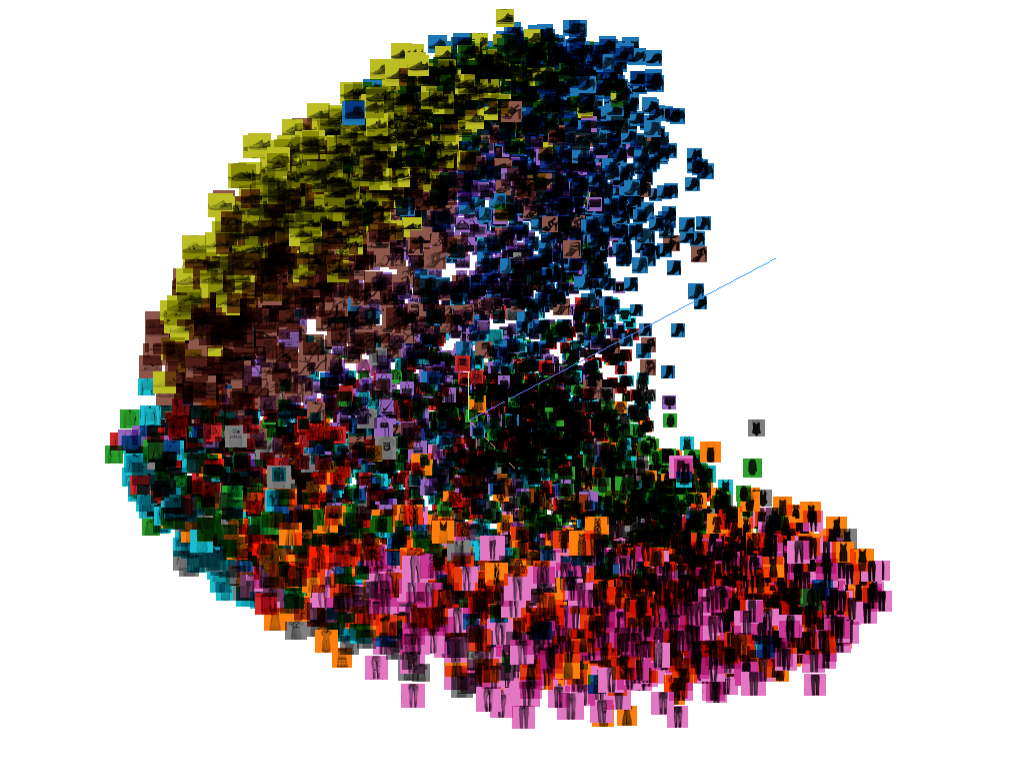
\includegraphics[scale=.15]{tensorboard_pca.png}
  \caption{Tensorboard visualization of the Fashion-MNIST dataset.}
  \label{fig:tensorboard_pca}
\end{figure}

\par We decided to use the Fashion-MNIST dataset created by Zalando Research due to the excellent documentation on Github and plethora of utilities available within their Github repository. The dataset consists of a training set and validation set. The training set contains 60,000 images while the validation set contains 10,000 images. Each image is a $28 \times 28$ grayscale image (784 total pixels). The training set is of the form $X = Y$, where $X$ is a $60,000 \times 784$ matrix and $Y$ is a $60,000 \times 1$ matrix. Each row in $X$ corresponds to a different image and each column corresponds to a pixel of that image (used as features). The $Y$ matrix is $60,000 \times 1$ matrix where each value is a classification for the corresponding row (image) in the $X$ matrix. Each classification is an integer value which maps to one of 10 different clothing classes.
\par To better understand our dataset, we decided to visualize it using Tensorboard \cite{tensorboard} and Matplotlib \cite{matplotlib}. Our implementation for visualizing the data is located in the \textbf{visualization.py} file in the top-level directory. We opted for a Principal Component Analysis (PCA) to get a better idea of what clusters may exist amongst the data. We chose PCA because the data has a relatively high number of features (784), which is not easy to visualize. With PCA, we have access to the features the preserve the most variance in the data, and may offer some insight into how it can be organized. When loaded into the Tensorboard visualization suite we were able to observe images like in Figure \ref{fig:tensorboard_pca}. Once colored, it was evident that the data actually formed reasonable clusters. This led us to believe that data was reasonably separable, so we \textit{should} see fairly high classification rates with a model using the correct features. Ideally, we would learn which features these are using the neural networks. Using Matplotlib, we were also able to visualize a single image as shown in Figure \ref{fig:single_image}. Upon visualizing this image, it was obvious that we should normalize the data. Since each pixel is a value between 0 and 255, we decided to normalize the data by dividing each pixel by 255. This proved extremely helpful in getting better results from our neural networks.

\begin{figure}[h!]
\centering
  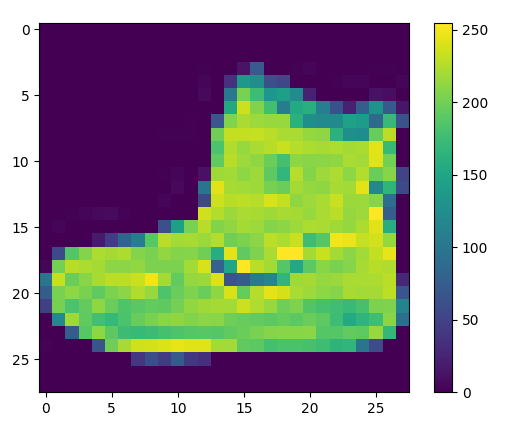
\includegraphics[scale=.33]{single_image.png}
  \caption{Image 0 from the Fashion-MNIST dataset visualized using a color map.}
  \label{fig:single_image}
\end{figure}

\section{Neural Network Configuration}

\par Our neural networks shared many of the same characteristics, as the only thing that needed to change between the CNN and FNN were the hidden layers between the input and output layers. 

\subsection{Activation Function}
Within these hidden layers we used the ReLU \cite{relu} activation function. 

\begin{eq} \label{eq:relu} 
    $$ f(x) = \left \{ 
    \begin{array}{rcl}
        0 & \mbox{for} & x < 0\\
        x & \mbox{for} & x \ge 0\end{array} \right. $$
\end{eq} 

The ReLU function works well because it is not expensive to compute, it doesn't contain any plateaus (so convergence is relatively quick), and it is sparsely activated. Sparse activation is a good thing in this scenario because it will increase the chance of a node not firing, and hence simulating a dropout effect to reduce overfitting. 

\subsection{Loss Function}

We decided to use the categorical cross-entropy loss function within our neural networks. 

\begin{eq} \label{eq:cceloss} 
    $$ L(y, \hat{y}) = - \sum_{j=0}^{M}\sum_{i=0}^{N}(y_{ij}\log{\hat{y}_{ij}}) $$
\end{eq} 

We wanted to use a loss function that returned a low value when the true value matched the value guessed by the model and a high value when the guess was not correct. In the categorical cross-entropy loss function there will only be contribution from a given term $y_i$ when $y_i \approx 1$, indicating a classification chosen by the algorithm. This classification will be correct when $\hat{y_i} \approx 1$, which will cause the overall term to approach zero (since $\log 1 = 0$). This loss function works very well for classification problems with multiple classes in general.

\subsection{Optimization Algorithm}

For our optimization algorithm we decided to go with Adam \cite{adam} because we wanted to try out one of the newer gradient descent variants produced by modern research. Adam was published in ICLR in 2015, and showed very promising training rates which we hoped to leverage in our project. The Adam algorithm can be used in Tensorflow applications through \texttt{tensorflow.keras.optimizers.Adam}.

\subsection{Metric}

To evaluate the testing and training performance of our neural networks we decided to use the typical classification accuracy formula:

\begin{eq} \label{eq:metric} 
    $$ A = \frac{1}{M} \sum_{i = 0}^{M} {(y_i = \hat{y_i})} $$
\end{eq} 

In the above formula, $M$ is the number of images in the training/test set that is being evaluated. The condition inside of the summation is used as shorthand to indicate the number of correct guesses. Essentially, this formula represents the number of correct guesses over the total number of items. We used this metric because we were familiar with it from class and there was support for it in Tensorflow.

\section{Convolutional Neural Network}

\section{Feedforward Neural Network}

\begin{figure}[h!] 
\centering
  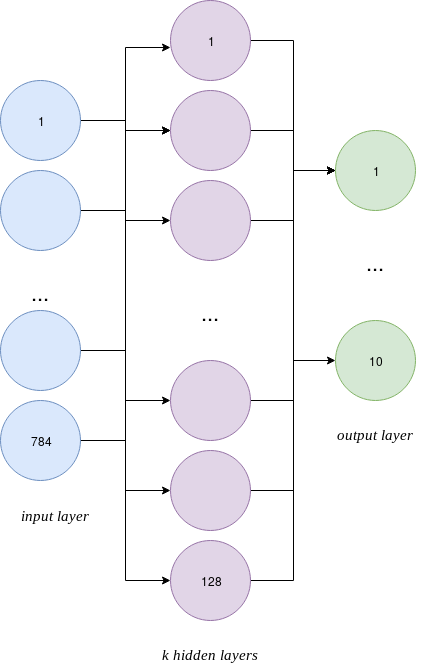
\includegraphics[scale=.33]{fNN.png}
  \caption{Diagram of our feedforward neural network design. The singular input layer
  contains 784 data points. There are \textit{k} hidden layers of 128 nodes each, and one output layer consisting of 10 data points}
  \label{fig:fnn_dia}
\end{figure}

Our feedforward neural network (FNN) took a $784 \times 1$ vector as input, representing the entire $28 \times 28$ image. Each pixel was normalized using the following function as determined in the data visualization stage:

$$ norm(x_i) = \frac{x_i}{255}$$

We thought the best way to fairly represent the feedforward neural network was to vary the capacity (variable $k$ in Figure \ref{fig:fnn_dia}), so in our experiments we tested with $k$ values of 1, 6, and 12. In testing these values we held the number of epochs at 20 to keep the training time low. With more time and better hardware we would have liked to increase the number of epochs to around 80. 

\section{Evaluation}

\subsection{Convolutional Neural Network}

\begin{figure}[h!] 
\centering
  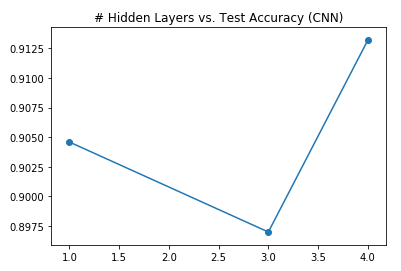
\includegraphics[scale=.5]{cNN_eval.png}
  \caption{Evaluation of the convolutional neural network with varying numbers of hidden layers.}
  \label{fig:fnn_dia}
\end{figure}


\subsection{Feedforward Neural Network}

\begin{figure}[h!] 
\centering
  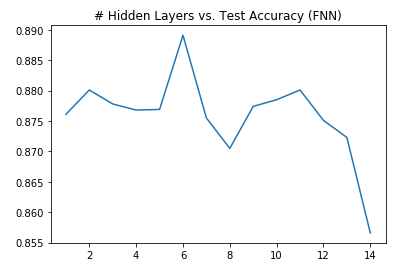
\includegraphics[scale=.5]{fNN_eval.png}
  \caption{Evaluation of the feedforward neural network with varying numbers of hidden layers.}
  \label{fig:fnn_dia}
\end{figure}


\section{Conclusion}

\section{Contributions}

\subsection{Matt}

Matt was responsible for organizing the Github repository, performing the data visualization phase (visualization.py), re-running experiments for the report, tuning hyperparameters for the FNN and CNN (experiments.ipynb), and for writing the majority of the report.

\subsection{Julius}

Julius was responsible for writing the first iteration of the experiment code (cNN.ipynb and fNN.ipynb) and writing preliminary results to the report.

\subsection{James}

James was responsible for investigating bootstrapping and cross-validation techniques for use in the neural networks.

\bibliographystyle{unsrt}
\bibliography{references}

\end{document}
